\section{Work Load Creation}
do I need to talk about system setup with EKS?
add another section for performance tuning?

== Starts with how locations are created
As explained in the \ref{ch:method}, timeseries has six primary attributes. In order to create a timeseries for performance testing, it needs data for each key attribute.
While generating the timeseries for performance testing, it selected locations all over the world as a generic case to include all the locations without binding to a specific area.

These locations https://developers.google.com/public-data/docs/canonical/countries\_csv are static though out the testing, and data added to the wdias-performance-test.
During the performance test, it creates 1000 timeseries and keep adding data against those timeseries. For each location, it creates four timeseries with vary with module Id key attribute with four values. Thus combining all together, those creates 1000 timeseries. But test cases generate these values before starts the performance tests, and able to increase the timeseries as wanted.

For grid data, it uses static 100 grid locations which based on how is \acrshort{api} exposed. Since grid locations have different metadata structure as described in \ref{se:db_struct}, those data handle separately. But the locationId of grid and scalar data types have the same effect when define a timeseries.

> Then using those, create timeseries metadata (how it assure 10% of Grid data)
In the \acrshort{jmeter} Best Practices, \say{If your test needs large amounts of data - particularly if it needs to be \emph{randomised} create the test data in a file that can be read with CSV Data set. This avoids wasting resources at run-time. jmeter best practices lean\_mean}. Rather providing the randomness in run time, the timeseries stored with the random order which satisfy the percentage of 70\% Scalar, 20\% Vector and 10\% Grid as mentioned in \ref{se:test_plan}.
Before running the test cases, it generate the metadata for timeseries and write into a CSV file which is shared among the threads in the \acrshort{jmeter}. This is occurred in the setup phase of the test cases. The metadata CSV file arrange in a way that within each 10 lines, 7 lines are Scalar timeseries, 2 lines are Vector timeseries, and 1 line is a Grid timeseries.

== Then how precipitation data for each time period created
The system is capable of storing any numeric value up to 3 decimal points. It does not make any different based on the parameter type whether it is the precipitation or the temperature. Thus during the performance testing, \acrshort{jmeter} is using real precipitation data from \acrshort{curw}. One month period of data for five weather stations have been using for prepare the test data. The script to cleanup and prepare the precipitation data is available as \emph{setup\_precipitation.sh} in wdias-performance.

\begin{lstlisting}[language=sh, caption=Precipitation Data Preparation]
Set ROOT_DIR=~/wdias/wdias-performance-test
-h | --help: Usage
  setup_precipitation.sh  <COMMAND>
    - COMMAND: help | extract | prepare | cleanup | populate
  e.g.
  setup_precipitation.sh prepare
    Segregate single file data into multiple files based on date. And Separate into main dirs of 15min, 30min, 60min and create tar files
  setup_precipitation.sh extract
    Extract the tar files into 15min, 30min and 60min
  setup_precipitation.sh cleanup
    Clean up extracted dirs
\end{lstlisting}
When preparing the data, it create three set of data based on the time interval such as hourly (60min), 30min, and 15min data with modifying the replicated data.
This will reduce the overhead in performance testing and increase the performance itself.
Extract function use while creating the containers, and extract the data into the container. This reduce the context loading while creating the container images.
While performing the load testing, \acrshort{jmeter} keep update a date counter, and create over the one month data. At the end of current month, the date counter advance to the next month. But data is repeat using from the beginning. In order to provide more randomness, it switch over five locations as well. The JSR223 scripts were written in a generic way such that is possible to tweak and use if there are more location data available.

> Then how water level data for Grid time series created
Almost similar to how was the precipitation data proceed, the water level are prepared for Grid data. One exception with Grid data during this test cases was, the maximum time step is 30min, instead of 15min due to larger size of the data. But the \acrshort{wdias} is capable of supporting such request. The main purpose of the \acrshort{wdias} is to provide a extensible architecture framework, during the performance testing it is not much consider about scaling the Grid data handling as it using \acrshort{netCDF}, and it is another domain with an attraction up to some extend.

\begin{lstlisting}[language=sh, caption=Water level Data Preparation]
Set ROOT_DIR=~/wdias/wdias-performance-test
-h | --help: Usage
  setup_water-level.sh  <COMMAND>
    - COMMAND: help | extract | prepare | cleanup | populate
  e.g.
  setup_water-level.sh prepare
    Segregate single file data into multiple grid file directories based on date. And Separate into main directories of 15min, 30min, 60min and create tar files
  setup_water-level.sh extract
    Extract the tar files into 15min, 30min and 60min
  setup_water-level.sh cleanup
    Clean up extracted directories
\end{lstlisting}
The water level also contains the real data for one month of period, and \emph{setup\_waterlevel.sh} script provide the functionality of prepare, cleanup and extract.
Also it reset and repeat reading from the beginning when the \acrshort{jmeter} date counter keep increasing.

> Talk about the test test up - JMeter
 -> mentioned distributed setup test data collect issue and continue with one server coz it can support what is required
\subsection{Experimental Setup}
In order to create higher work load using the \acrshort{jmeter}, it has Distributed Testing feature. It is using the master slave approach and it allowed to handle all the test cases via single instance, rather handling separate instances. But it has following limitation;
\say{Note: The same test plan is run by all the servers. JMeter does not distribute the load between servers, each runs the full test plan. So if you set 1000 Threads and have 6 JMeter server, you end up injecting 6000 Threads.}

\begin{figure}[htp]
    \centering
    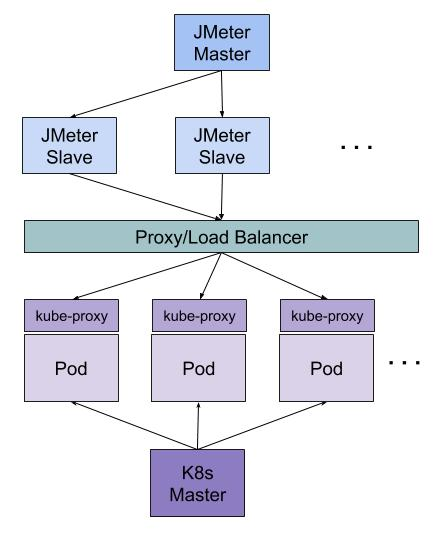
\includegraphics[width=0.6\textwidth]{results/work_load/experimental_setup_v3.jpg}
    \caption{Experimental Setup with JMeter}
    \label{fi:experimental_setup}
\end{figure}
\begin{figure}[htp]
    \centering
    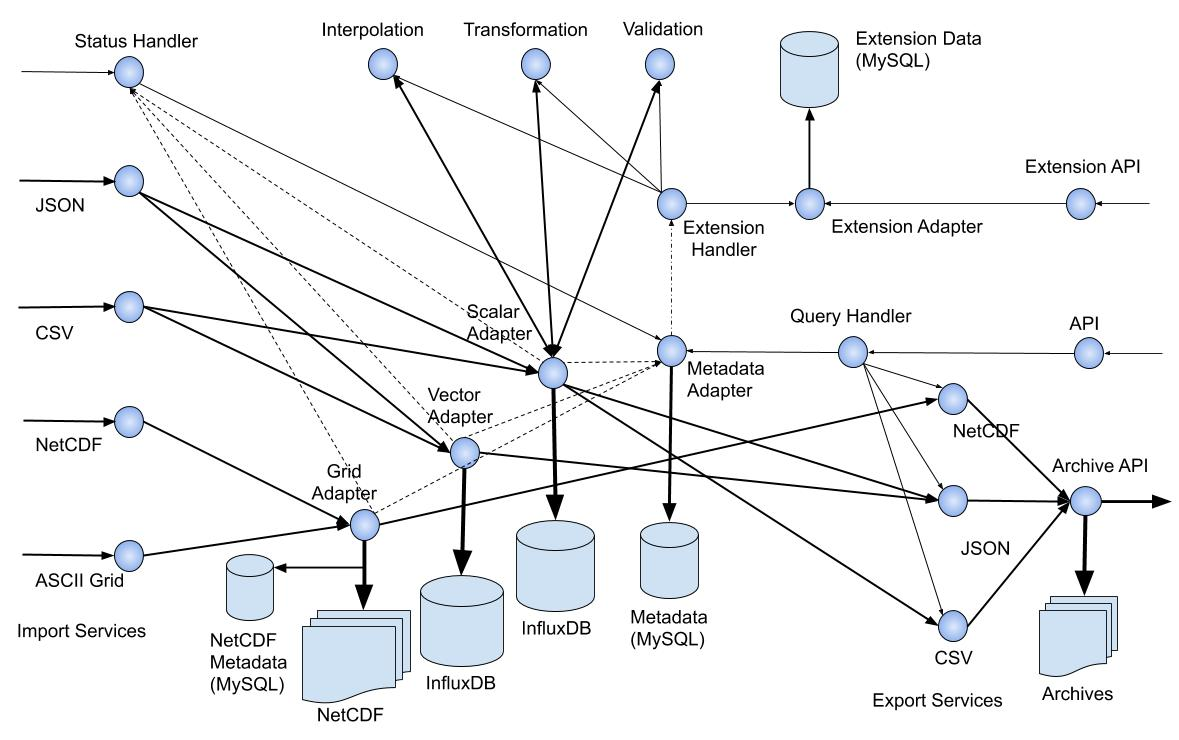
\includegraphics[width=1\textwidth]{method/microservice/microservice_architecture-handle_on_async-v3.jpg}
    \caption{Weather Data Integration and Assimilation System Architecture for Handle Request Asynchronously}
    \label{fi:wdias_micro_async}
\end{figure}

> Talk about Stepping timer with concurrent thread group


> Add screenshot of jmeter setup
> Add prod req graph
> talk about how test cases are enabled
> talk about test plans can run
\begin{lstlisting}[language=sh, caption=Test Plan Help]
-h | --help: Usage
    <ROOT_DIR> <COMMAND> <REQ_SIZE>
    - REQ_SIZE (optional): 24(1) | 288(2) | 1044(3)
  NOTE: Modify test.conf as necessary
  e.g.
  test_plan.sh ~/wdias/wdias-performance-test run
  test_plan.sh ~/wdias/wdias-performance-test run 2
  - Run all the steps in order of setup, import, 
    create_extension, extension, export, all, query

  test_plan.sh ~/wdias/wdias-performance-test setup
  test_plan.sh ~/wdias/wdias-performance-test import 24
  test_plan.sh ~/wdias/wdias-performance-test create_extension 24
  test_plan.sh ~/wdias/wdias-performance-test extension 24
  test_plan.sh ~/wdias/wdias-performance-test export 24
  test_plan.sh ~/wdias/wdias-performance-test all 24
  test_plan.sh ~/wdias/wdias-performance-test query 24

  Distributed Mode
  SERVER_IPS=<IP1,IP2...> test_plan.sh ~/wdias/wdias-performance-test run

\end{lstlisting}

> JMeter performance tuning
  Use CSV files rather Random generates
  Use JSR223 scripts with Grrovy
  Using Stepping Timer
  

